% ==== Document Class & Packages =====
\documentclass[12pt,hidelinks]{article}
	\usepackage[explicit]{titlesec}
	\usepackage{titletoc}
	\usepackage{tocloft}
	\usepackage{charter}
	\usepackage[many]{tcolorbox}
	\usepackage{amsmath}
	\usepackage{graphicx}
	\usepackage{xcolor}
	\usepackage{tikz,lipsum,lmodern}
	\usetikzlibrary{calc}
	\usepackage[english]{babel}
	\usepackage[utf8]{inputenc}
	\usepackage{fancyhdr}
	\usepackage{mathrsfs}
	\usepackage{empheq}
	\usepackage{fourier}% change to lmodern if fourier is no available
	\usepackage{wrapfig}
	\usepackage{fancyref}
	\usepackage{hyperref}
	\usepackage{cleveref}
	\usepackage{listings}
	\usepackage{varwidth}
	\usepackage{longfbox}
	\usepackage{geometry}
	\usepackage{marginnote}
	\usepackage{setspace}
	\usepackage{subfigure}
	\usepackage{minted}
	\tcbuselibrary{theorems}
	\tcbuselibrary{breakable, skins}
	\tcbuselibrary{listings, documentation}
	\geometry{
		a4paper,
		left=33mm,
		right=33mm,
		top=20mm}
% ========= Path to images ============
%   - Direct the computer on the path 
% 	  to the folder containg the images
% =====================================
\graphicspath{{./images/}}
% ============= Macros ================
\newcommand{\fillin}{\underline{\hspace{.75in}}{\;}}
\newcommand{\solution}{\textcolor{mordantred19}{Solution:}}
\setlength{\parindent}{0pt}
\addto{\captionsenglish}{\renewcommand*{\contentsname}{Table of Contents}}
\linespread{1.2}
% ======== Footers & Headers ==========
\cfoot{\thepage}
\chead{}\rhead{}\lhead{}
% =====================================
\renewcommand{\thesection}{\arabic{section}}
\newcommand\sectionnumfont{% font specification for the number
	\fontsize{380}{130}\color{myblueii}\selectfont}
\newcommand\sectionnamefont{% font specification for the name "PART"
	\normalfont\color{white}\scshape\small\bfseries }
% ============= Colors ================
% ----- Red -----
\definecolor{mordantred19}{rgb}{0.68, 0.05, 0.0}
% ----- Blue -----
\definecolor{st.patrick\'sblue}{rgb}{0.14, 0.16, 0.48}
\definecolor{teal}{rgb}{0.0, 0.5, 0.5}
\definecolor{beaublue}{rgb}{0.74, 0.83, 0.9}
\definecolor{mybluei}{RGB}{0,173,239}
\definecolor{myblueii}{RGB}{63,200,244}
\definecolor{myblueiii}{RGB}{199,234,253}
% ---- Yellow ----
\definecolor{blond}{rgb}{0.98, 0.94, 0.75}
\definecolor{cream}{rgb}{1.0, 0.99, 0.82}
% ----- Green ------
\definecolor{emerald}{rgb}{0.31, 0.78, 0.47}
\definecolor{darkspringgreen}{rgb}{0.09, 0.45, 0.27}
% ---- White -----
\definecolor{ghostwhite}{rgb}{0.97, 0.97, 1.0}
\definecolor{splashedwhite}{rgb}{1.0, 0.99, 1.0}
% ---- Grey -----
\definecolor{whitesmoke}{rgb}{0.96, 0.96, 0.96}
\definecolor{lightgray}{rgb}{0.92, 0.92, 0.92}
\definecolor{floralwhite}{rgb}{1.0, 0.98, 0.94}
% ========= Part Format ==========
\titleformat{\section}
{\normalfont\huge\filleft}
{}
{20pt}
{\begin{tikzpicture}[remember picture,overlay]
	\fill[myblueiii] 
	(current page.north west) rectangle ([yshift=-13cm]current page.north east);   
\node[
	fill=mybluei,
	text width=2\paperwidth,
	rounded corners=6cm,
	text depth=18cm,
	anchor=center,
	inner sep=0pt] at (current page.north east) (parttop)
	{\thepart};%
\node[
	anchor=south east,
	inner sep=0pt,
	outer sep=0pt] (partnum) at ([xshift=-20pt]parttop.south) 
	{\sectionnumfont\thesection};
\node[
	anchor=south,
	inner sep=0pt] (partname) at ([yshift=2pt]partnum.south)   
	{\sectionnamefont SECTION};
\node[
	anchor=north east,
	align=right,
	inner xsep=0pt] at ([yshift=-0.5cm]partname.east|-partnum.south) 
	{\parbox{.7\textwidth}{\raggedleft#1}};
\end{tikzpicture}%
}
% ========= Hyper Ref ===========
\hypersetup{
	colorlinks,
	linkcolor={red!50!black},
	citecolor={blue!50!black},
	urlcolor={blue!80!black}
}
% ========= Example Boxes =============
\tcbset{
	defstyle/.style={
		fonttitle=\bfseries\upshape, 
		fontupper=\slshape,
		arc=0mm, 
		beamer,
		colback=blue!5!white,
		colframe=blue!75!black},
	theostyle/.style={
		fonttitle=\bfseries\upshape, 
		fontupper=\slshape,
		colback=red!10!white,
		colframe=red!75!black},
	visualstyle/.style={
		height=6.5cm,
		breakable,
		enhanced,
		leftrule=0pt,
		rightrule=0pt,
		bottomrule=0pt,
		outer arc=0pt,
		arc=0pt,
		colframe=mordantred19,
		colback=lightgray,
		attach boxed title to top left,
		boxed title style={
			colback=mordantred19,
			outer arc=0pt,
			arc=0pt,
			top=3pt,
			bottom=3pt,
		},
		fonttitle=\sffamily,},
	discussionstyle/.style={
		height=6.5cm,
		breakable,
		enhanced,
		rightrule=0pt,
		toprule=0pt,
		outer arc=0pt,
		arc=0pt,
		colframe=mordantred19,
		colback=lightgray,
		attach boxed title to top left,
		boxed title style={
			colback=mordantred19,
			outer arc=0pt,
			arc=0pt,
			top=3pt,
			bottom=3pt,
		},
		fonttitle=\sffamily},
	mystyle/.style={
		height=6.5cm,
		breakable,
		enhanced,
		rightrule=0pt,
		leftrule=0pt,
		bottomrule=0pt,
		outer arc=0pt,
		arc=0pt,
		colframe=mordantred19,
		colback=lightgray,
		attach boxed title to top left,
		boxed title style={
			colback=mordantred19,
			outer arc=0pt,
			arc=0pt,
			top=3pt,
			bottom=3pt,
		},
		fonttitle=\sffamily},
	aastyle/.style={
			height=3.5cm,
			enhanced,
			colframe=teal,
			colback=lightgray,
			colbacktitle=floralwhite,
			fonttitle=\bfseries,
			coltitle=black,
		attach boxed title to top center={
	  		yshift=-0.25mm-\tcboxedtitleheight/2,
	   		yshifttext=2mm-\tcboxedtitleheight/2}, 
		boxed title style={boxrule=0.5mm,
			frame code={ \path[tcb fill frame] ([xshift=-4mm]frame.west)
				-- (frame.north west) -- (frame.north east) -- ([xshift=4mm]frame.east)
				-- (frame.south east) -- (frame.south west) -- cycle; },
			interior code={ 
				\path[tcb fill interior] ([xshift=-2mm]interior.west)
				-- (interior.north west) -- (interior.north east)
				-- ([xshift=2mm]interior.east) -- (interior.south east) -- (interior.south west)
				-- cycle;} }
				},
	examstyle/.style={
		height=9.5cm,
		breakable,
		enhanced,
		rightrule=0pt,
		leftrule=0pt,
		bottomrule=0pt,
		outer arc=0pt,
		arc=0pt,
		colframe=mordantred19,
		colback=lightgray,
		attach boxed title to top left,
		boxed title style={
			colback=mordantred19,
			outer arc=0pt,
			arc=0pt,
			top=3pt,
			bottom=3pt,
		},
		fonttitle=\sffamily},
	doc head command={
		interior style={
			fill,
			left color=yellow!20!white, 
			right color=white}},
	doc head environment={
		boxsep=4pt,
		arc=2pt,
		colback=yellow!30!white,
		},
	doclang/environment content=text
}
% ============= Boxes ================
\newtcolorbox[auto counter,number within=section]{example}[1][]{
	mystyle,
	title=Example~\thetcbcounter,
	overlay unbroken and first={
		\path
		let
		\p1=(title.north east),
		\p2=(frame.north east)
		in
		node[anchor=
			west,
			font=\sffamily,
			color=st.patrick\'sblue,
			text width=\x2-\x1] 
		at (title.east) {#1};
	}
}
\newtcolorbox[auto counter,number within=section]{longexample}[1][]{
	examstyle,
	title=Example~\thetcbcounter,
	overlay unbroken and first={
		\path
		let
		\p1=(title.north east),
		\p2=(frame.north east)
		in
		node[anchor=
		west,
		font=\sffamily,
		color=st.patrick\'sblue,
		text width=\x2-\x1] 
		at (title.east) {#1};
	}
}
\newtcolorbox[auto counter,number within=section]{example2}[1][]{
	aastyle,
	title=Example~\thetcbcounter,{}
}
\newtcolorbox[auto counter,number within=section]{discussion}[1][]{
	discussionstyle,
	title=Discussion~\thetcbcounter,
	overlay unbroken and first={
		\path
		let
		\p1=(title.north east),
		\p2=(frame.north east)
		in
		node[anchor=
		west,
		font=\sffamily,
		color=st.patrick\'sblue,
		text width=\x2-\x1] 
		at (title.east) {#1};
	}
}
\newtcolorbox[auto counter,number within=section]{visualization}[1][]{
	visualstyle,
	title=Visualization~\thetcbcounter,
	overlay unbroken and first={
		\path
		let
		\p1=(title.north east),
		\p2=(frame.north east)
		in
		node[anchor=
		west,
		font=\sffamily,
		color=st.patrick\'sblue,
		text width=\x2-\x1] 
		at (title.east) {#1};
	}
}
% --------- Theorems ---------
\newtcbtheorem[number within=subsection,crefname={definition}{definitions}]%
	{Definition}{Definition}{defstyle}{def}%
\newtcbtheorem[use counter from=Definition,crefname={theorem}{theorems}]%
	{Theorem}{Theorem}{theostyle}{theo}
	%
\newtcbtheorem[use counter from=Definition]{theo}{Theorem}%
{
	theorem style=plain,
	enhanced,
	colframe=blue!50!black,
	colback=yellow!20!white,
	coltitle=red!50!black,
	fonttitle=\upshape\bfseries,
	fontupper=\itshape,
	drop fuzzy shadow=blue!50!black!50!white,
	boxrule=0.4pt}{theo}
\newtcbtheorem[use counter from=Definition]{DashedDefinition}{Definition}%
 {
 	enhanced,
 	frame empty,
 	interior empty,
 	colframe=darkspringgreen!50!white,
	coltitle=darkspringgreen!50!black,
	fonttitle=\bfseries,
	colbacktitle=darkspringgreen!15!white,
	borderline={0.5mm}{0mm}{darkspringgreen!15!white},
	borderline={0.5mm}{0mm}{darkspringgreen!50!white,dashed},
	attach boxed title to top center={yshift=-2mm},
	boxed title style={boxrule=0.4pt},
	varwidth boxed title}{theo}
%%%%%%%%%%%%%%%%%%%%%%%%%%%%%%%%%%%%%%%%
\newtcblisting[auto counter,number within=section]{disexam}{
	skin=bicolor,
	colback=white!30!beaublue,
	colbacklower=white,
	colframe=black,
	before skip=\medskipamount,
	after skip=\medskipamount,
	fontlower=\footnotesize,
	listing options={style=tcblatex,texcsstyle=*\color{red!70!black}},}
%%%%%%%%%%%%%%%%%%%%%%%%%%%%%%%%%%%%%%%

\begin{document}
\begin{titlepage}
	\centering % Center everything on the title page
	\scshape % Use small caps for all text on the title page
	\vspace*{1.5\baselineskip} % White space at the top of the page
% ===================
%	Title Section 	
% ===================

	\rule{13cm}{1.6pt}\vspace*{-\baselineskip}\vspace*{2pt} % Thick horizontal rule
	\rule{13cm}{0.4pt} % Thin horizontal rule
	
		\vspace{0.75\baselineskip} % Whitespace above the title
% ========== Title ===============	
	{	\Huge Dspace\\ 
			\vspace{4mm}
		MANUAL  \\	}
% ======================================
		\vspace{0.75\baselineskip} % Whitespace below the title
	\rule{13cm}{0.4pt}\vspace*{-\baselineskip}\vspace{3.2pt} % Thin horizontal rule
	\rule{13cm}{1.6pt} % Thick horizontal rule
	
		\vspace{1.75\baselineskip} % Whitespace after the title block
% =================
%	Information	
% =================
	{\large Leonard \\
		\vspace*{1.2\baselineskip}
	EMAIL: leonardcampelo@ibict.br} \\
	\vfill
If you come across any problems, see section \ref{sec:resources} for possible\\ \vspace{1mm}
solutions or contact me at \url{armindubert19@gmail.com}\\ \vspace{1mm}
Happy \LaTeX-ing!
\end{titlepage}
%%%%%%%%%%%%%%%%%%%%%%%%%%%%%%%%%%%%%%%%%%%%%%%%%%%%%%%%%%%
\tableofcontents
\vfill
\small{\noindent \textbf{About This File} \vspace{-3mm}\\
\noindent \rule{3.3cm}{0.5pt} \\
This file was created for the benefit of all teachers and students wanting to use Latex for tests/exams/lessons/thesis/articles etc.\\
The entirety of the contents within this file, and folder, are free for public use.}
\newpage
\newgeometry{
	left=29mm, 
	right=29mm, 
	top=20mm, 
	bottom=15mm}
%%%%%%%%%%%%%%%%%%%%%%%%%%%%%%%%%%%%%%%%%%%%%%%%%%%%%%%%%%%
\section{Introdução}
\newpage
    \subsection{O que é o DSpace?}
        Para que serve?
        DSpace é um software de código-fonte aberto que fornece facilidades para o gerenciamento de acervo digital, utilizado para implementação de repositórios institucionais. Suporta uma grande variedade de tipo de documentos, tais como: livros, teses e dissertações, fotografias, filmes, áudio, e outros. Os documentos são organizados em comunidades e coleções.
        O DSpace é disponibilizado livremente às instituições de investigação, sob a forma de um produto de código aberto, que pode ser livremente adaptado e expandido funcionalmente, nos termos da Licença BSD Open source license.

    \subsection{Especificações técnicas do sistema}
        A Recomendação mínima recomendada para um pequeno servidor:
        
    \singlespacing \textbullet \hspace{6pt} 2 GB de memória RAM
 
    \textbullet \hspace{6pt} 40 GB de disco rígido
 
    \textbullet \hspace{6pt} Placa de rede on-board
 
    \textbullet \hspace{6pt} Processador de único núcleo, com 2.6 GHz

    \singlespacing  O DSpace utiliza os seguintes software para operar um servidor e cada um deles utiliza uma política de uso da documentação específica. Abaixo segue uma lista com os software: 
 
    \singlespacing \textbullet \hspace{6pt} Apache Ant, http://ant.apache.org/manual/index.html
  
    \textbullet \hspace{6pt} Apache Maven 3.0.5 ou superior (3.3.9 +), https://maven.apache.org/index.html
  
    \textbullet \hspace{6pt} Apache Tomcat 7 ou 8, http://tomcat.apache.org/
 
    \textbullet \hspace{6pt} JDK 7 ou 8(64-bit) http://openjdk.java.net/install/

\newpage
\section{Instalação}
\newpage
\begin{enumerate}
    
    \item \textbf{Crie o usuário do DSpace:} 
    
        \begin{minted}{bash}
useradd -m dspace
        \end{minted}
    
        \begin{minted}{bash}
passwd dspace
        \end{minted}
    
   
    \item \textbf{Execute a atualização dos pacotes do seu sistema operacional:} 
    
        \begin{minted}{bash}
apt-get update && apt-get upgrade -y
        \end{minted}
   
    \item \textbf{Execute o seguinte comando para Instalar o OpenJDK 7 ou OpenJDK8. Esteja ciente de que o Tomcat 7 usa o Java 1.6 para compilar JSPs por padrão . O Tomcat 8 usa o Java 1.7 para JSPs por padrão . Se você usar outro Container Servlet, consulte sua documentação sobre este assunto.}
     
        \begin{minted}{bash}
apt-get install openjdk-7-jdk
        \end{minted}\\
        
        ou
    
        \begin{minted}{bash}
apt-get install openjdk-8-jdk
        \end{minted}\\       
        
    \item \textbf{Instale o Apache Maven 3.0.5 ou superior (3.3.9 +) * (ferramenta de compilação Java)}\\
        \begin{enumerate}
            \item O Apache-Maven é a ferramenta que realiza a construção de toda a árvore de pacotes que serão necessários para instalação do DSpace, e além disso compila o código fonte, deixando-o pronto para instalação. Para a instalação do Apache-Maven, deve-se baixar o seu pacote binário no endereço http://maven.apache.org/ e descompactá-lo, estando dentro da /home/dspace/ por meio do comando (x.x.x representa o número da versão baixada):
        \end{enumerate}
        
            \texttt{tar -vzxf apache-maven-x.x.x-bin.tar.gz}\\
        
        
    \item \textbf{ Instale o Apache Ant 1.8 ou posterior (ferramenta de compilação Java)}\\
         \begin{enumerate}
            \item A ferramenta que executa a tarefa de instalação do DSpace é o Apache-Ant. Para tornar esse software disponível para uso, basta realizar o download de seu pacote binário em http://ant.apache.org/ e descompactá-lo dentro da /home/dspace.\\
            
                \texttt{tar -vzxf apache-ant-x.x.x-bin.tar.gz}\\
            
            \item \textbf{Ou então se preferir, execute:}\\
                \begin{minted}{bash}
apt-get install ant
                \end{minted}
            
        \end{enumerate}
        
        \item \textbf{Instale o Apache-Tomcat, é o servidor Web que torna disponível o acesso do DSpace via rede (seja a Intranet ou a Internet).} \\
    
        
        \begin{enumerate}
            \item Para instalá-lo basta baixar seu pacote binário em http://tomcat.apache.org/ e descompactá-lo dentro da /home/dspace. (O Tomcat 8.0.32 encontrado, por exemplo, no Debian 9 Stretch e Ubuntu 16.04 Xenial ) tem um bug que causará PropertyBatchUpdateException ou StringIndexOutOfBoundsException.   Isto foi corrigido em 8.0.33. Se você estiver usando o Tomcat 7, recomendamos executar o Tomcat 7.0.30 ou superior. Tomcat 7.0.29 e versões inferiores sofrem um vazamento de memória. Como resultado, essas versões do tomcat requerem uma quantidade incomum de memória para executar o DSpace. Isso foi resolvido a partir do Tomcat 7.0.30.)
        \end{enumerate}
        
                \texttt{tar -vzxf apache-tomcat.xxxx.tar.gz} \\
        
        \item \textbf{Baixe o DSpace customizado pelo IBICT do GitHub e jogue no diretório do dspace:}\\
        
            \texttt{cd /home/dspace/}\\
        
        \item \textbf{Descompacte o arquivo:}\\
        
            \texttt{unzip repositorio-padrao-dspace-6\_\textbf{x}.zip}\\
            
        \item \textbf{Instale o Git (na verdade não é usado com este método, mas resolve um erro produzido pelo maven):}\\    
            
            \begin{minted}{bash}
apt-get install git
            \end{minted}
            
        \item \textbf{Instale o PostgreSQL 9.6: (versões anteriores do PostgreSQL <9.4 podem não funcionar corretamente com o DSpace, por causa da extensão do pgcrypto):}\\
            
        \begin{minted}{bash}
sh -c 'echo "deb http://apt.postgresql.org/pub/repos/apt/ 
`lsb_release -cs`-pgdg main" >> /etc/apt/sources.list.d/pgdg.list'
        \end{minted}

       \begin{minted}{bash}
wget -q https://www.postgresql.org/media/keys/ACCC4CF8.asc -O - | apt-key add -
       \end{minted}
      
       \begin{minted}{bash}
apt-get update
       \end{minted}
            
        \begin{minted}{bash}
apt-get install postgresql-9.6 postgresql-contrib-9.6
       \end{minted}


        \item \textbf{Vamos fazer o login no PostgreSQL e criar o banco de dados e o usuário do banco de dados do DSpace:}\\
        
            \begin{minted}{bash}
su - postgres
            \end{minted}
            
            \begin{minted}{bash}
createuser --username=postgres --no-superuser --pwprompt dspace
            \end{minted}
            
            \begin{minted}{bash}
createdb --username=postgres --owner=dspace --encoding=UNICODE dspace
            \end{minted}
            
            \begin{minted}{bash}
psql --username=postgres dspace -c "CREATE EXTENSION pgcrypto;"
            \end{minted}
            
             \begin{minted}{bash}
exit
            \end{minted}
            
        \item \textbf{Agora devemos adicionar uma linha ao PostgreSQL para autenticação do cliente:}\\
    
        \begin{enumerate}
            \item Abra o arquivo pg\_hba.conf com seu editor favorito (nano, vi, etc.)\\
            
                \texttt{nano /etc/postgresql/9.6/main/pg\_hba.conf}\\

            \item E adicione a seguinte linha\\
            
                \texttt{local     all     dspace    md5}\\
                
             \item Reinicie o PostgreSQL para adotar as mudanças\\
            
                \texttt{/etc/init.d/postgresql restart}\\

            \end{enumerate}
            
        \item \textbf{Certifique-se que o diretório destino de instalação está com permissões de escrita ao usuário dspace, deve-se logar como root e executar o comandos:}\\
        
            \texttt{mkdir /dspace-base}
            
             \begin{minted}{bash}
chown -R dspace:dspace /dspace-base/
            \end{minted}
            
            \begin{minted}{bash}
chown -R dspace:dspace /home/dspace/
            \end{minted}
            
        \item \textbf{Todos comandos a seguir devem ser executados com o usuário dspace, salvo se explicitado o login de root.}\\
        
        \item \textbf{Entre na pasta DSpace-fonte.  Será necessário que se realize uma cópia do local.cfg EXAMPLE para local.cfg. Localizado em: DSpace/config/local.cfg.exemple.}\\
        
            \texttt{cp local.cfg.EXAMPLE local.cfg}\\
            
        \item \textbf{Não esqueça de entrar no arquivo local.cfg. E Preencher o campo do dspace.install.dir como dspace-base}\\
            
            \texttt{dspace.install.dir=/dspace-base}\\
        
        \item \textbf{Comandos para executar o maven:}\\
        
            \texttt{cd repositorio-padrao-dspace-6\_x/}\\
            
             \begin{minted}{bash}
/home/dspace/apache-maven-x.x.x/bin/mvn -U package
            \end{minted}
            
            \begin{enumerate}
            \item Após aproximadamente 30 min, o sistema deve responder com um log na tela, e ao final a mensagem BUILD SUCCESSFUL.\\

            \end{enumerate}
            
        \item \textbf{O próximo é o apache Ant:}\\
        
         \begin{enumerate}
            \item Caso tenha baixado o pacote binário. Com o usuário dspace, a instalação deve ser executada dentro do DSpace-fonte/dspace/target/dspace-installer, e é realizada por meio do comando.\\
            
                \begin{minted}{bash}
/home/dspace/apache-ant-x.x.x/bin/ant fresh_install\\
            \end{minted}
            
            \item Se tiver baixado o pacote pelo apt-get install ant, siga os seguintes passos:\\
            
            \texttt{cd dspace/target/dspace-installer}\\
            
            \begin{minted}{bash}
ant fresh_install
            \end{minted}

            \end{enumerate}
            
        \item \textbf{Finalizada a instalação do apache-Ant. Faça as modificações necessárias no arquivo dspace.cfg. Localizado em /dspace-base/config. Este arquivo é composto dos parâmetros de configuração do dspace. Segue uma tabela descritiva dos principais variáveis a serem configuradas:}
            
        \begin{figure}[!ph]
            \centering
            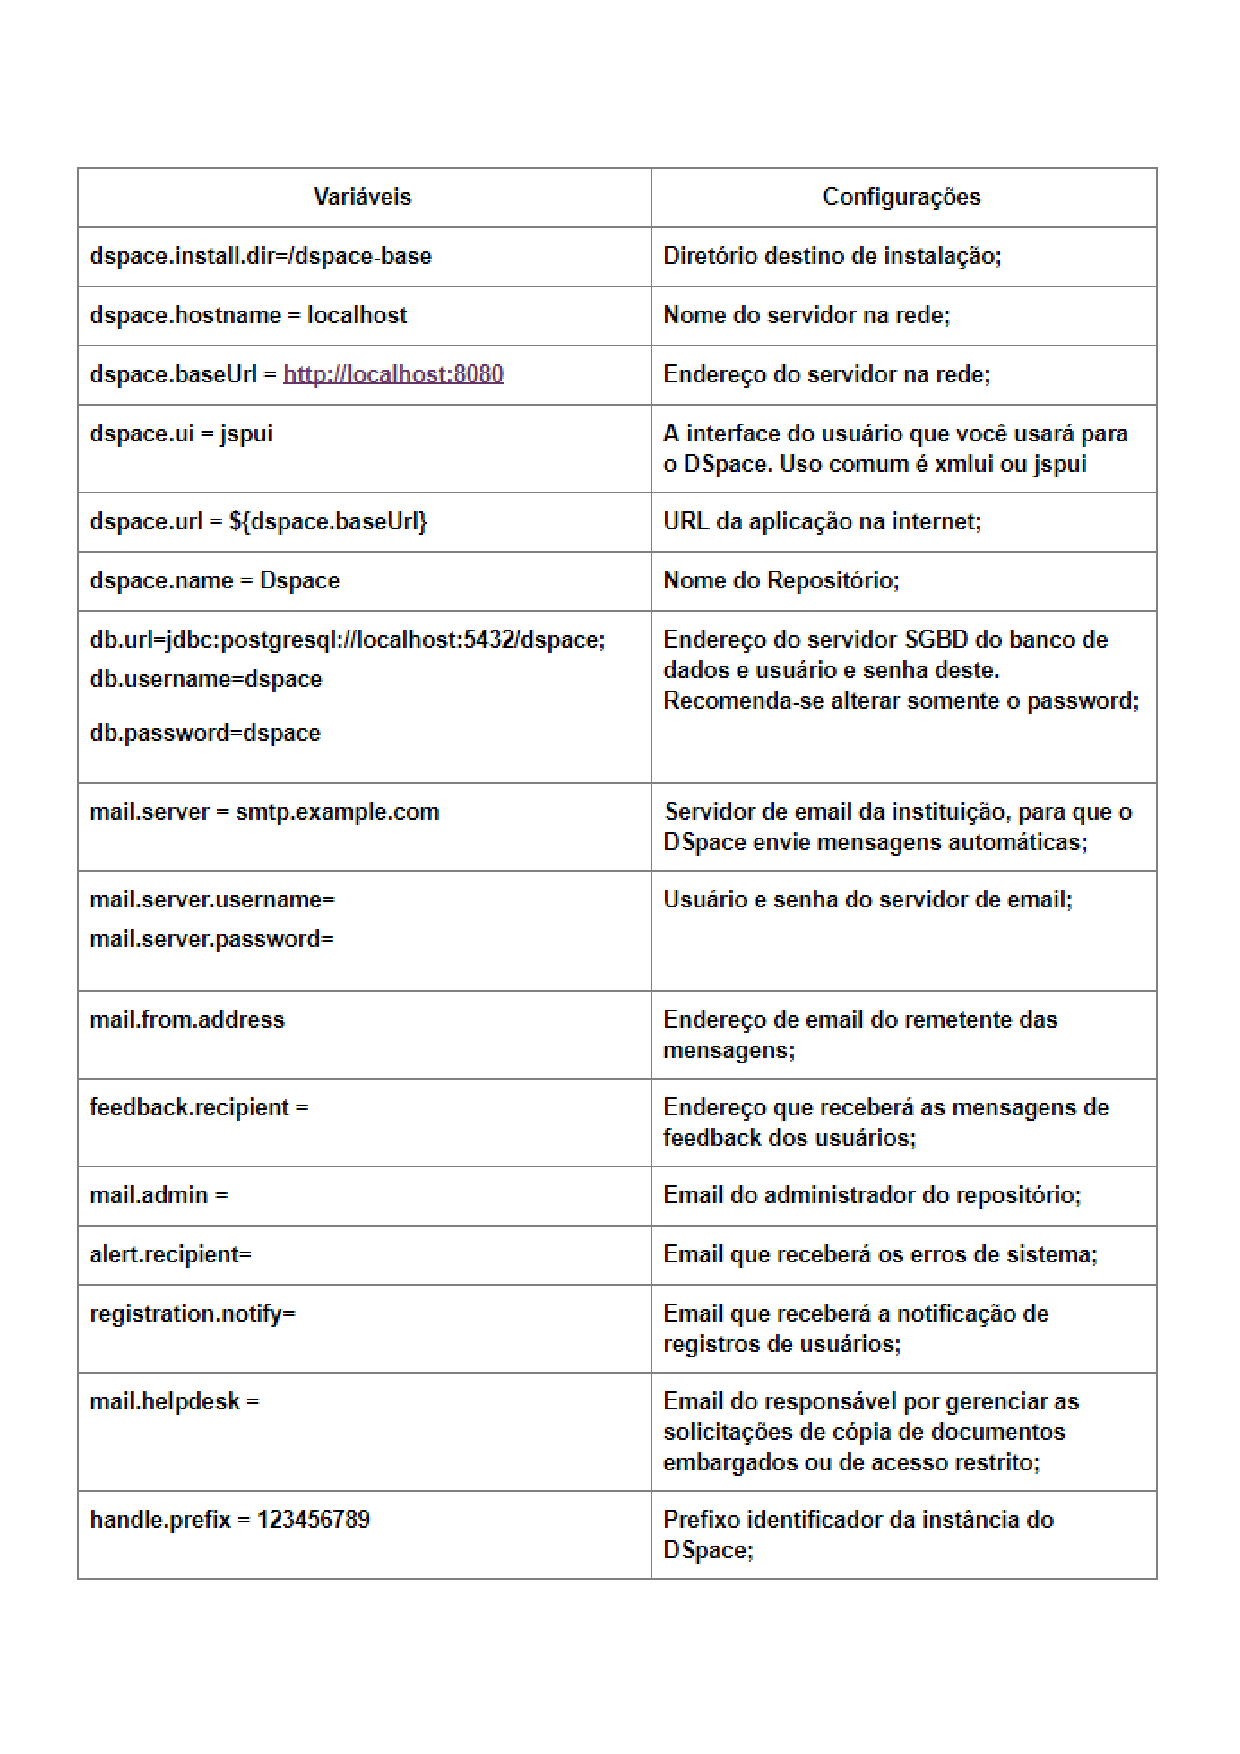
\includegraphics[scale=0.7]{figura/variaveis.pdf}
            \caption{Tabela das configurações básicas.}
        \label{Rotulo}
        \end{figure}
        
        
        \newpage

        \item \textbf{Finalizada a instalação do apache-Ant. Faça as modificações necessárias no arquivo dspace.cfg. Localizado em /dspace-base/config. Este arquivo é composto dos parâmetros de configuração do dspace. Segue uma tabela descritiva dos principais variáveis a serem configuradas:}
        
            \texttt{<Connector port="8080" protocol="HTTP/1.1"\\
                    connectionTimeout="20000"\\
                    redirectPort="8443" URIEncoding="UTF-8" />}\\
            
        
        \item \textbf{A ativação do servidor Web Apache-Tomcat com a aplicação do DSpace se dá por meio dos comandos. E deve ser executada dentro encontra /dspace-base/webapps:}\\
            
         \begin{minted}{bash}
cp -R jspui/ solr/ oai/  /home/dspace/apache-tomcat-x.x.x/webapps/
         \end{minted}
         
          \item \textbf{Este último expande os parâmetro de memória reservada para o Apache-Tomcat. Contudo, se o servidor for reiniciado, essa configuração será perdida. Para torná-la definitiva, edite o arquivo que se encontra em home/dspace/apache-tomcat-x.x.x/bin/catalina.sh e adicione ao final dele as linhas:}\\
          
            \begin{minted}{bash}
JAVA_OPTS="-Djava.awt.headless=true -Xms512M -Xmx768M -XX:MaxPermSize=256M 
-XX:+UseParallelGC -XX:MaxGCPauseMillis=1500 -XX:GCTimeRatio=9 -server
-XX:+DisableExplicitGC"
            \end{minted}
         
         \item \textbf{Por fim, com o usuário dspace basta que se inicie o servidor Apache-Tomcat:}\\

            \begin{minted}{bash}
/home/dspace/apache-tomcat-x.x.x/bin/startup.sh
            \end{minted}
            
        \item \textbf{Em seguida, crie o administrador do DSpace. Após a instalação do DSpace é necessário que se crie uma senha de administrador, o que pode ser feito pelo comando:}\\
        
            \begin{minted}{bash}
/dspace-base/bin/dspace create-administrator
            \end{minted}
            
        \item \textbf{Agora você pode acessar a página principal do DSpace JSPUI em:}\\
        
        \begin{minted}{bash}
http://localhost:8080/jspui
            \end{minted}

\end{enumerate}

\newpage
\section{Configurações básicas}
\newpage
      \subsection{Protocolo oai}\\
 
      É por meio do protocolo OAI-PMH que é feita a coleta dos Repositórios, Bibliotecas e Revistas para o Portal brasileiro de publicações científicas em acesso aberto (oasisbr) <http://oasisbr.ibict.br/vufind/>  e a Biblioteca Digital Brasileira de Teses e Dissertações (BDTD) <http://bdtd.ibict.br/vufind/>. Devem ser feito os devidos apontamentos neste arquivo para o perfeito funcionamento da url de coleta.\\
      
      Localizado em \textbf{/dspace-base/config/modules/oai.cfg} 

          \begin{figure}[!htp]
                \centering
                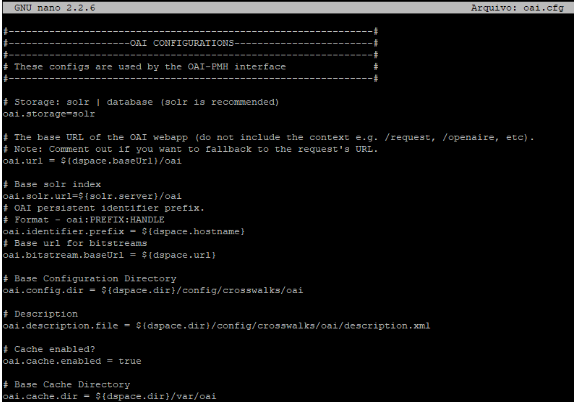
\includegraphics[scale=0.9]{figura/oai.png}
                \caption{Arquivo oai.cfg.}
            \label{Rotulo}
          \end{figure}
        
    \subsection{Ativação da url oai}\\
   
    Em sua instalação padrão, o OAI está disponível dentro da pasta \textbf{[dspace-base]/webapps/oai/} da instalação do DSpace. E para sua ativação, deve-se seguir os seguintes passos:
        
        
        \begin{enumerate}
            \item Copiar as pastas \textbf{[dspace-base]/webapps/oai/} e \textbf{[dspace-base]/webapps/solr/} para dentro da webapps, do servidor de aplicação Apache-Tomcat;
            
            \item Reiniciar o servidor Apache-Tomcat;
            
            \item Executar o comando:\\
             \texttt{[dspace-base]/bin/dspace oai import -c -v}\\
             \texttt{[dspace-base]/bin/dspace oai clean-cache}

        \end{enumerate}
        
\newpage
    \subsection{Sincronização automática da url OAI do repositório}\\
    Ainda é necessário que se inclua alguns comandos na \textbf{contrab} do sistema, que é uma forma de agendar algumas tarefas que deverão ser executadas durante o período em que o uso do sistema pela comunidade não seja tão intenso. Esse procedimento pode ser efetuado, quando se está logado como root, se executa o comando: \textbf{crontab -e}. Após abertura do arquivo da crontab, devem ser adicionadas as seguintes linhas, informando o usuário dspace, os caminhos e os comandos no final do documento:
    
    \begin{minted}{bash}
0 0 * * * dspace /dspace-base/bin/dspace oai import
    \end{minted}

\newpage
\section{Formulário de entrada}
\newpage
    \subsection{O que é o Formulário de entrada?}
O formulário de entrada é utilizado para determinar a estrutura dos metadados que serão usados para descrever os documentos durante o processo de submissão.
\singlespacing
Em linguagem mais simples e no contexto dos repositórios, os metadados são os campos que serão preenchidos para descrever o objeto digital que está sendo submetido.
É um arquivo em XML (eXtensible Markup Language) composto por campos (indicados pela tag <field>) que podem ser adequados aos tipos de documentos contidos no repositório, ou seja, você pode configurar o formulário para que este contenha os metadados necessários de acordo com o tipo de documento a ser depositado.
\singlespacing
Essa configuração não pode ser feita através da interface gráfica, sendo necessário o auxílio de equipe com conhecimento técnico do DSpace para que seja executada.
O endereço do arquivo que permite a edição do formulário é o \textbf{[dspace-base]/config/input-forms.xml}. Para registrar novos metadados no DSpace é necessário inseri-los também via interface.

        \begin{figure}[!htp]
                \centering
                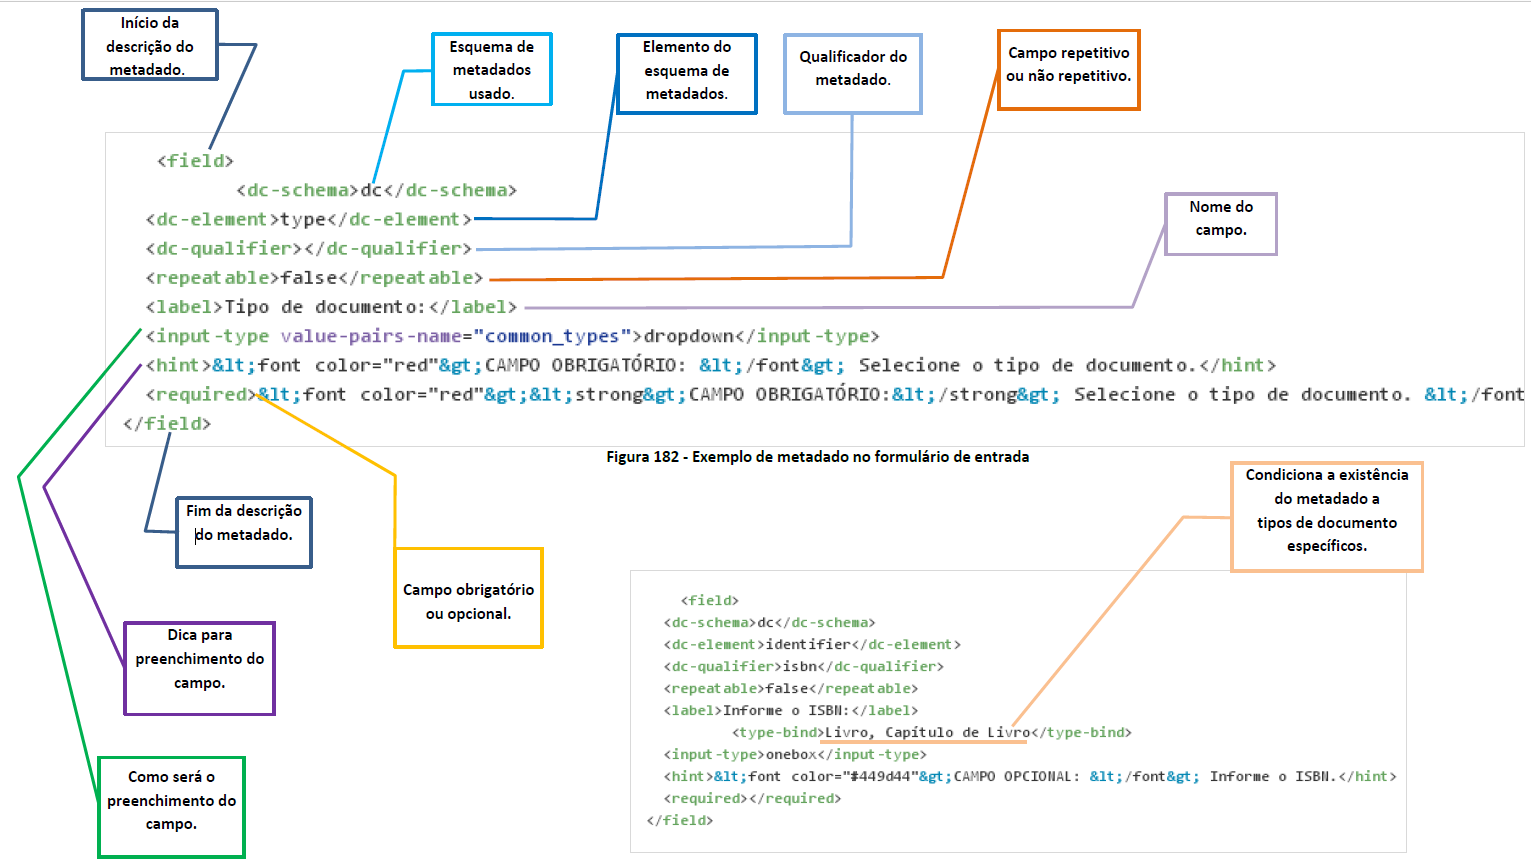
\includegraphics[scale=0.4]{figura/input-forms.png}
                \caption{Formulário de entrada}
            \label{Rotulo}
          \end{figure}
\newpage
    \subsection{Registrar metadados}
Para registrar novos metadados no DSpace é necessário inseri-los tanto via interface, o que será mostrado abaixo, quanto no formulário de entrada. Por padrão o DSpace utiliza uma versão qualificada do esquema Dublin Core. É possível também configurar outros esquemas de metadados no registro.
\singlespacing
Passo 1: Para registrar novos metadados ou alterar vá no menu do Administrador e em “Configurações gerais” e clique na opção <Registrar metadados>.
    
        \begin{figure}[!htp]
                \centering
                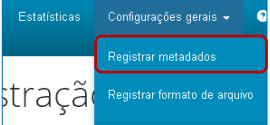
\includegraphics[scale=0.9]{figura/registrar-metadados-passo1.png}
                \caption{Registrar-metadados-passo-1}
            \label{Rotulo}
        \end{figure}

Passo 2: A página seguinte apresenta a lista dos esquemas registrados. Como será adicionado um metadado no Dublin Core (dc), clique no primeiro link como mostrado na figura abaixo.

         \begin{figure}[!htp]
                \centering
                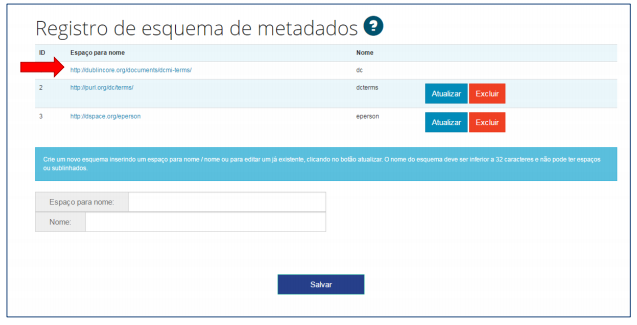
\includegraphics[scale=0.9]{figura/registrar-metadados-passo2.png}
                \caption{Registrar-metadados-passo-2}
            \label{Rotulo}
        \end{figure}
\newpage
Passo 3: Na página seguinte é fornecida uma lista dos metadados registrados, separando elementos e qualificadores e os comentários. É possível atualizar ou excluir esses metadados, clicando respectivamente em “Atualizar” ou “Excluir”. Para adicionar novo metadado, vá até o fim da página
        \begin{figure}[!htp]
                \centering
                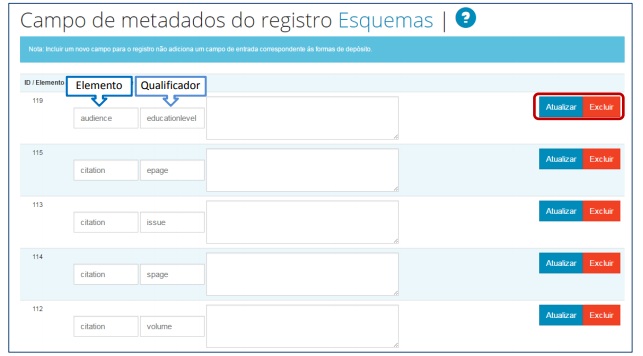
\includegraphics[scale=0.9]{figura/registrar-metadados-passo3.png}
                \caption{Registrar-metadados-passo-3}
            \label{Rotulo}
        \end{figure}

Passo 4: Em “Adicionar campo de metadado”, preencha os campos “Elemento”, “Qualificador” e “Nota de Escopo”. O preenchimento do qualificador e da nota de escopo não é obrigatório e pode ser deixado em branco. O qualificador quando preenchido NÃO pode conter espaços ou sublinhados. Depois de preenchido, clique em “Adicionar novo” e o metadado será criado.

        \begin{figure}[!htp]
                \centering
                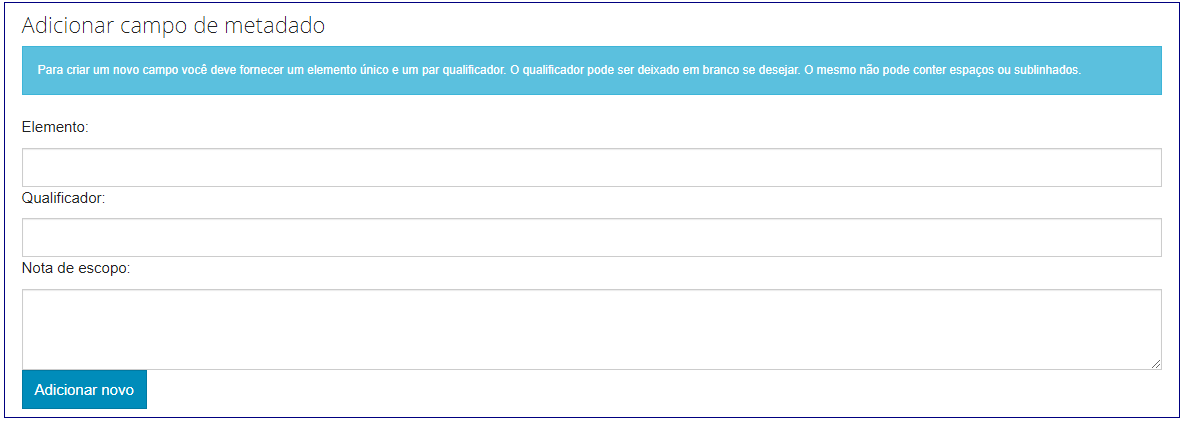
\includegraphics[scale=0.5]{figura/registrar-metadados-passo4.png}
                \caption{Registrar-metadados-passo-4}
            \label{Rotulo}
        \end{figure}

\newpage
\section{Upgrade de versões}
\newpage
\subsection{Upgrade de versões}
Realizar upgrade de versões não é uma tarefa simples e direta. Há alguns dificultadores, os mais comuns são:\\

\textbullet \hspace{6pt} Migrar as configurações antigas para a nova versão;\\
\textbullet \hspace{6pt} Migrar arquivos de layout que foram alterados pelo usuário;\\
\textbullet \hspace{6pt} Migrar as estatísticas antigas do solr;\\
\textbullet \hspace{6pt} Atualizar a base de dados;\\
\textbullet \hspace{6pt} Migrar a assetstore (pasta que contém os documentos);
\singlespacing
É possível perceber uma diferença entre os procedimentos descritos no manual oficial do DSpace 6.x e o que aqui se apresenta. De fato, entende-se que existe maior segurança em se realizar uma instalação clean da nova versão e se aplicar nela as configurações particulares da antiga. Essa tarefa gera também uma melhor compreensão do processo de atualização, e é possível estabelecer um procedimento genérico de migração de uma versão 1.x ou 3.x para a 6.x.
\singlespacing
Para melhor entender como é feita a atualização de versões, a figura abaixo descreve, de forma simples, os passos explicados nessa página:

\subsection{Backup}
Para o backup da base de dados basta que se execute o comando:

\begin{minted}{bash}
pg_dump dspace4x > bkp_dspace4x_DDMMAA.sql
\end{minted}

Já para o backup da(s) pasta(s) assetstore, basta que se execute o comando, para cada pasta utilizada (em geral só se utiliza uma única pasta, que deve estar dentro da pasta base de instalação. Contudo para se ter certeza de qual(is) pasta(s) é(são) utiliza(s), deve-se verificar no arquivo \textbf{dspace-4.x-base/config/dspace.cfg} os parâmetros \textbf{assetstore.dir, assetstore.dir.1 e assetstore.dir.2}, estando dentro da pasta dspace-4.x-base:   

\begin{minted}{bash}
tar -cvzf bkp_assetstore_DDMMAA.tar.gz assetstore
\end{minted}

O backup das estatísticas pode ser feito, dentro da pasta dspace-4.x-base/solr/, com:

\begin{minted}{bash}
tar -cvzf bkp_solr_DDMMAA.tar.gz data
\end{minted}

\subsection{Restore}

\textbf{Base de dados}
\singlespacing
\textbullet \hspace{6pt} Remova e crie novamente a base de dados da nova instalação. Isso fornecerá uma base de dados vazia:

\begin{minted}{bash}
dropdb dspace6x
\end{minted}

\begin{minted}{bash}
createdb -E UNICODE dspace6x
\end{minted}

\textbullet \hspace{6pt} Para que possamos realizar o restore, vá até o local onde está o arquivo backup do banco e execute o comando:

\begin{minted}{bash}
psql -d dspace6x -f bkp_dspace4x_DDMMAA.sql
\end{minted}

\newpage
\subsection{Assetstore}

\textbullet \hspace{6pt} Mova o arquivo backup da(s) assetstore(s) para dentro da pasta \textbf{dspace-6.x-base}, e lá execute o comando:

\begin{minted}{bash}
tar -vzxf bkp_assetstore_DDMMAA.tar.gz
\end{minted}

\subsection{Estatísticas}

\textbullet \hspace{6pt} Mova o arquivo backup da(s) assetstore(s) para dentro da pasta \textbf{dspace-6.x-base}, e lá execute o comando:

\begin{minted}{bash}
tar -vzxf bkp_solr_DDMMAA.tar.gz
\end{minted}

Para atualizar os índices execute, dentro da pasta dspace-6.x-base/bin, os comandos:
\begin{minted}{bash}
./dspace index-discovery -f
\end{minted}

\newpage
\section{Layout}
\newpage

\subsection{home.jsp}

Uma parte crítica de qualquer atualização são as mudanças de layout. É necessário ter conhecimento de quais arquivos foram alterados, e sobrescrevê-los na interface de usuário jspui. 

Para fazer as alterações na página principal o arquivo para tal finalidade é o home.jsp

        \begin{figure}[!htp]
                \centering
                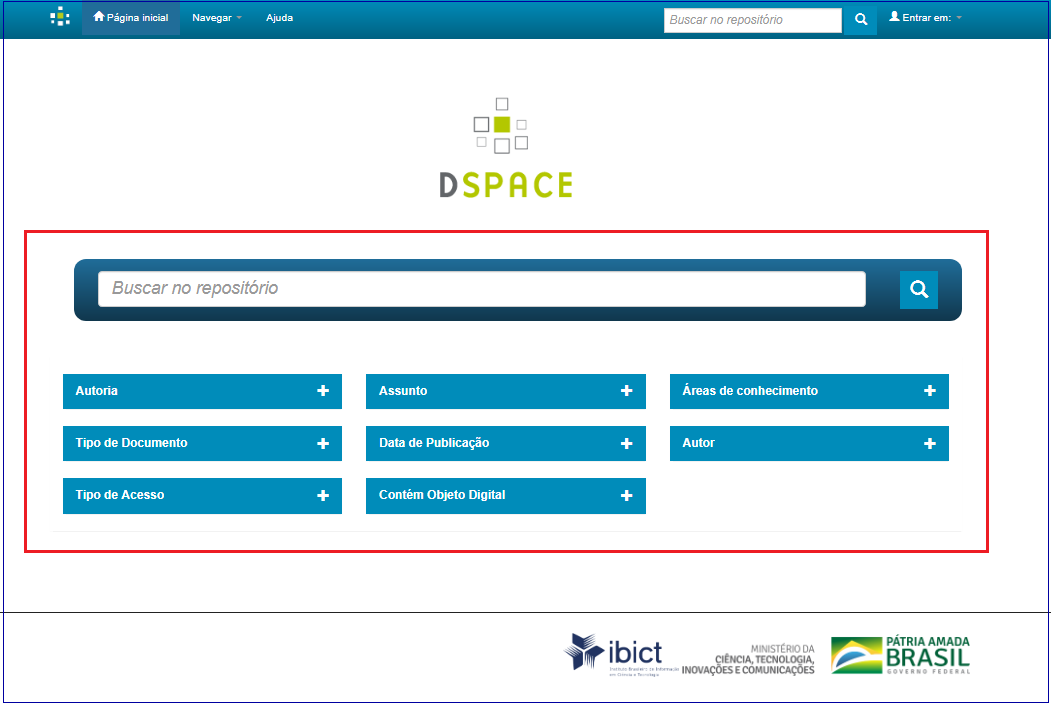
\includegraphics[scale=0.5]{figura/home.png}
                \caption{home.jsp}
            \label{Rotulo}
        \end{figure}

\subsection{navbar-default.jsp}
Para as alterações na página que se encontra no topo você deve se atentar para o navbar-default.jsp.

\begin{figure}[!htp]
                \centering
                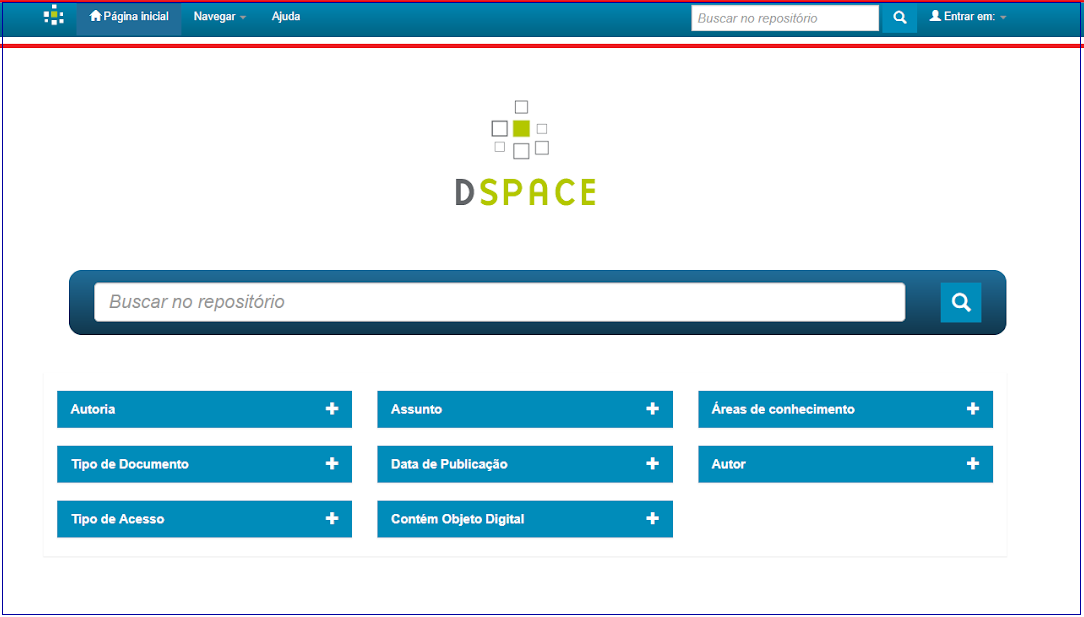
\includegraphics[scale=0.5]{figura/navbar-default.png}
                \caption{navbar-default.jsp}
            \label{Rotulo}
        \end{figure}

\newpage  

\subsection{Webui-browse-index}

Para a inclusão dos metadados na barra do “navegar”. 

    \begin{figure}[!htp]
        \centering
        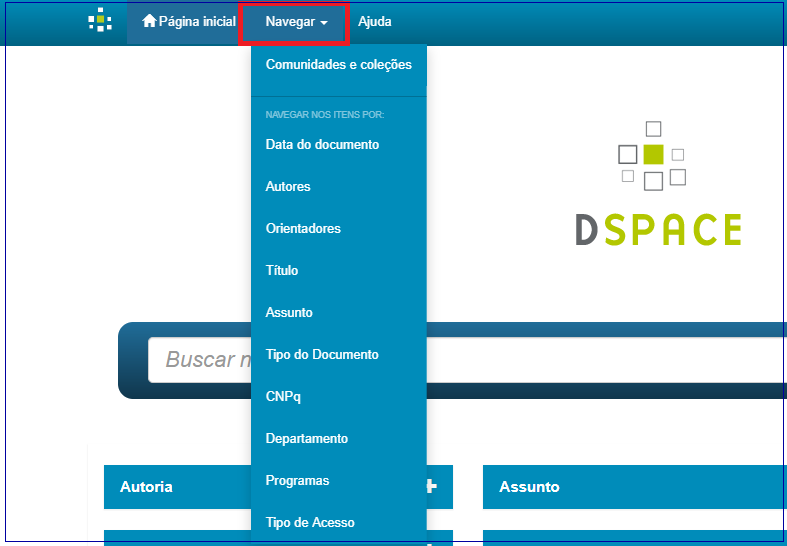
\includegraphics[scale=0.5]{figura/navegar1.png}
        \caption{navbar-default.jsp}
        \label{Rotulo}
     \end{figure}



É feita no arquivo dspace.cfg, localizado em /dspace-base/config/ e são incluídas nas variáveis webui.browse.index


    \begin{figure}[!htp]
        \centering
        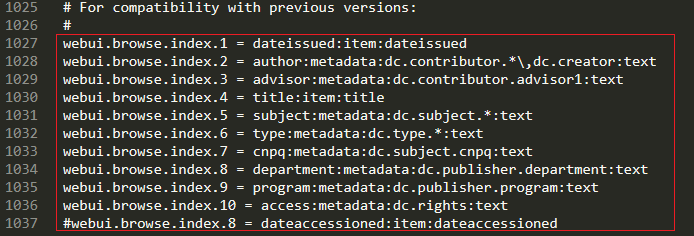
\includegraphics[scale=0.5]{figura/webui-browse-index.png}
        \caption{navbar-default.jsp}
        \label{Rotulo}
    \end{figure}
 
\newpage
\subsection{Inclusão das imagens}
       
Para a inclusão da imagem que se encontra no topo.

\begin{figure}[!htp]
        \centering
        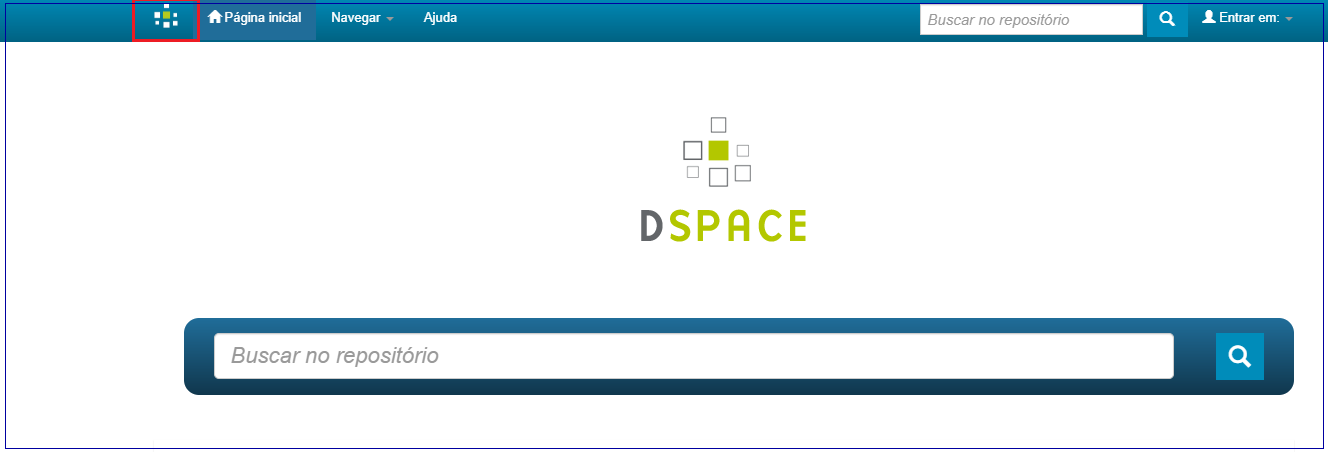
\includegraphics[scale=0.5]{figura/logo-topo.png}
        \caption{navbar-default.jsp}
        \label{Rotulo}
    \end{figure}
    
A imagem tem que ser adicionada em \textbf{/home/dspace/apache-tomcat/jspui/image/}  
\singlespacing
Assim como, tem que ser informado o caminho da imagem nos arquivos navbar-admin.jsp e navbar-default.jsp, que ficam localizadas em: \textbf{/home/dspace/apache-tomcat-x.x.x/webapps/jspui/layout/}  

\begin{figure}[!htp]
        \centering
        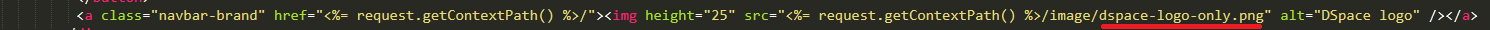
\includegraphics[scale=0.3]{figura/dspace-logo-only1.png}
        \label{Rotulo}
    \end{figure}
    
\begin{figure}[!htp]
        \centering
        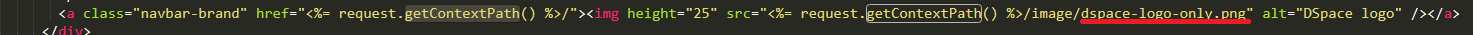
\includegraphics[scale=0.3]{figura/dspace-logo-only2.png}
        \caption{navbar-admin.jsp e navbar-default.jsp}
        \label{Rotulo}
    \end{figure}

Em relação a inclusão da logo principal.
\begin{figure}[!htp]
        \centering
        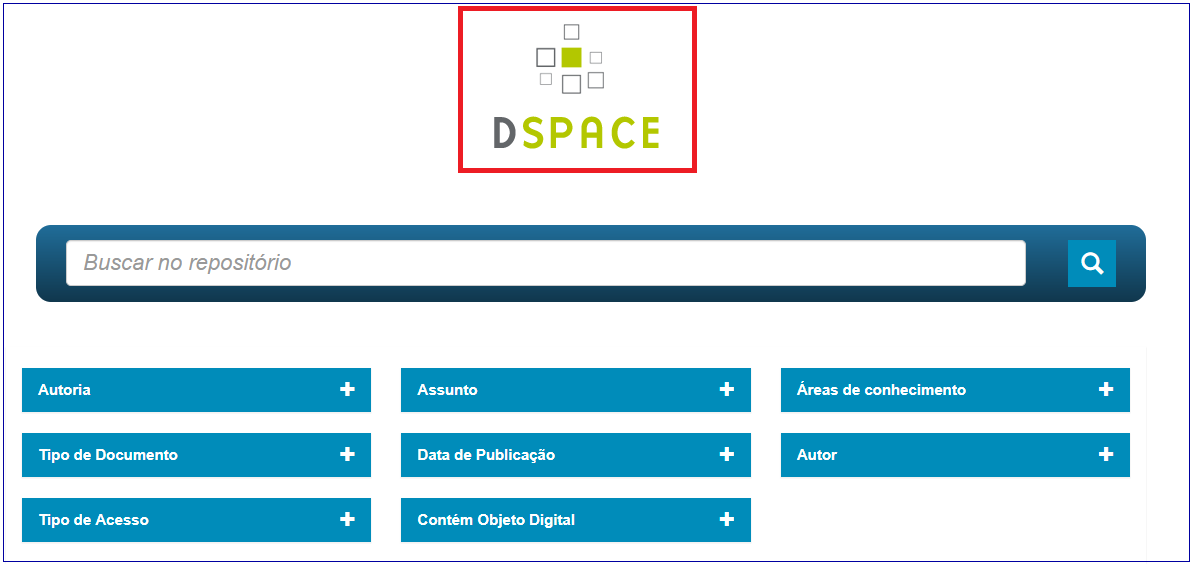
\includegraphics[scale=0.5]{figura/logo-principal.png}
        \caption{}
        \label{Rotulo}
    \end{figure}
    
\newpage 
A imagem tem que ser adicionada em \textbf{/home/dspace/apache-tomcat/jspui/image/} 
Assim como, tem que ser informado o caminho da imagem no arquivo header-default.jsp, que fica localizado em:  \textbf{/home/dspace/apache-tomcat-x.x.x/webapps/jspui/layout/}
    \begin{figure}[!htp]
        \centering
        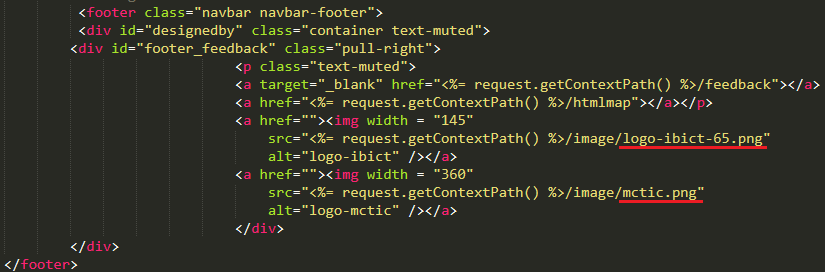
\includegraphics[scale=0.5]{figura/footer-default.png}
        \caption{footer-default.jsp}
        \label{Rotulo}
    \end{figure}
    
\end{document}